\chapter{Membangun Model Prediksi}

% Untuk pratikum saati ini menggunakan buku \textit{Python Artificial Intelligence Projects for Beginners}\cite{eckroth2018python}. Dengan praktek menggunakan python 3 dan editor anaconda dan library python scikit-learn.
% Dataset ada di https://github.com/PacktPublishing/Python-Artificial-Intelligence-Projects-for-Beginners .
% Tujuan pembelajaran pada pertemuan pertama antara lain:
% \begin{enumerate}
% \item
% Mengerti implementasi klasifikasi
% \item
% Memahami data set, training dan testing data
% \item
% Memahami Decission tree.
% \item
% Memahami information gain dan entropi.
% \end{enumerate}
% Tugas dengan cara dikumpulkan dengan pull request ke github dengan menggunakan latex pada repo yang dibuat oleh asisten riset. Kode program menggunakan input listing ditaruh di folder src ekstensi .py dan dipanggil ke latex dengan input listings. Tulisan dan kode tidak boleh plagiat, menggunakan bahasa indonesia yang sesuai dengan gaya bahasa buku teks.

\section{Teori}
Praktek teori penunjang yang dikerjakan(nilai 5 per nomor, untuk hari pertama) :
\begin{enumerate}
\item
Jelaskan apa itu binary classification dilengkapi ilustrasi gambar sendiri\\
Binary classification adalah proses mengklasifikasi yang ouputnya dibagi menjadi 2 kelas 

\item
Jelaskan apa itu supervised learning dan unsupervised learning dan clustering dengan ilustrasi gambar sendiri.
\par
    \textit{Supervised Learning} sebuah pembelajaran yang ditentukan berdasarkan penggunaan traning set yang berlabel.
\par
    \textit{Unsupervised Learning} sebuah pembelajaran yang ditentukan berdasarkan penggunaan traning set yang tidak berlabel. 

\item
Jelaskan apa itu evaluasi dan akurasi dari buku dan disertai ilustrasi contoh dengan gambar sendiri
\par
    Evaluasi adalah tentang mengukur sebarapa baik nilai performa dari suatu model. Dan akurasi adalah tigkat ketepatan yang benar dari suatu model.
    
\item
Jelaskan bagaimana cara membuat dan membaca confusion matrix, buat confusion matrix buatan sendiri.\\
Cara membuat dan membaca confusion matrix :
\begin{enumerate}
    \item Tentukan studi kasus nya
    \item Buat ke dalam Decision Tree
    \item Siapkan data testing 
    \item Kemudian cari value dari variabel misal nya a,b,c,d
    \item Dan cari value dari recall, precision, accuracy dan juga error state
\end{enumerate}

\item
Jelaskan bagaimana K-fold cross validation bekerja dengan gambar ilustrasi contoh buatan sendiri.
Cara kerja dari K-fold cross validation :
\begin{enumerate}
    \item Total instace dibagi menjadi n bagian
    \item Fold pertama merupakan bagian pertama yang menjadi Testing data dan sisanya menjadi training data
    \item Hitung akurasinya dengan menggunakan persamaan
    \item Fold ke dua merupakan bagian kedua yang menjadi testing data dan sisanya mendjadi training data
    \item Hitung lagi akurasi nya dan juga seterus nya pada fold yang terakhir
    \item Dan terakhir adalah hitung rata-rata akurasi nya
\end{enumerate}
\begin{figure}[!htbp]
    \centering
    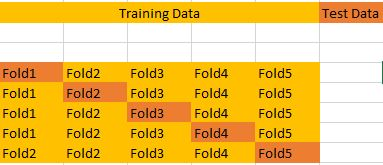
\includegraphics[scale=0.5]{figures/K-fold.JPG}
	\caption{Ilutrasi K-fold cross validation}
\end{figure}


\item
Jelaskan apa itu decision tree dengan gambar ilustrasi contoh buatan sendiri.\\
Decision Tree adalah suatu metode yang digunakan untuk mengambil keputusan


\item
Jelaskan apa itu information gain dan entropi dengan gambar ilustrasi buatan sendiri.\\
information gain adalah kumpulan informasi yang diperolah dari variable acak. Dan Entropi adalah tingkat keacakan pada informasi yang sedang diproses.\\



\end{enumerate}

\section{scikit-learn}
Dataset ambil di https://github.com/PacktPublishing/Python-Artificial-Intelligence-Projects-for-Beginners folder Chapter01.
Tugas anda adalah, dataset ganti menggunakan \textbf{student-mat.csv} dan mengganti semua nama variabel dari kode di bawah ini dengan nama-nama makanan (NPM mod 3=0), kota (NPM mod 3=1), buah (NPM mod 3=2), . Jalankan satu per satu kode tersebut di spyder dengan menggunakan textit{Run current cell}. Kemudian Jelaskan dengan menggunakan bahasa yang mudah dimengerti dan bebas plagiat dan wajib skrinsut dari komputer sendiri masing masing nomor di bawah ini(nilai 5 masing masing pada hari kedua).

\begin{enumerate}

\item load dataset student-mat.csv
\begin{figure}[!htbp]
    \centering
    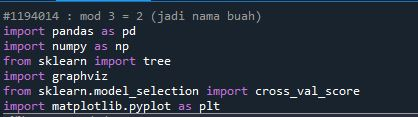
\includegraphics[scale=0.5]{figures/importchap2.JPG}
	\caption{Import}
    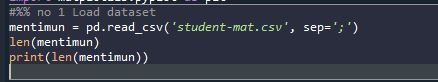
\includegraphics[scale=0.5]{figures/Chap2-1.JPG}
	\caption{Source Code Task 1}
    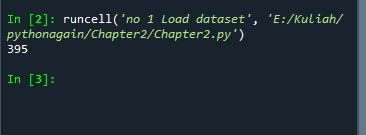
\includegraphics[scale=0.5]{figures/Chap2-1.1.JPG}
	\caption{Hasil Task}
\end{figure}

\newpage
\item generate binary label
\begin{figure}[!htbp]
    \centering
    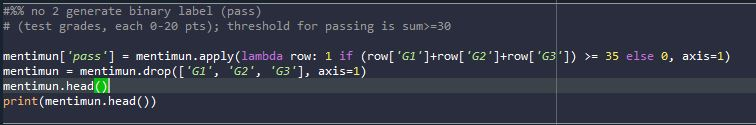
\includegraphics[scale=0.4]{figures/Chap2-2.JPG}
	\caption{Source Code Task 2}
    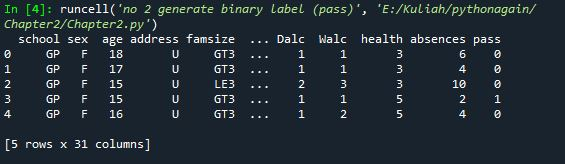
\includegraphics[scale=0.5]{figures/Chap2-2.1.JPG}
	\caption{Hasil Task 2}
\end{figure}

\item use one-hot encoding on categorical columns
\begin{figure}[!htbp]
    \centering
    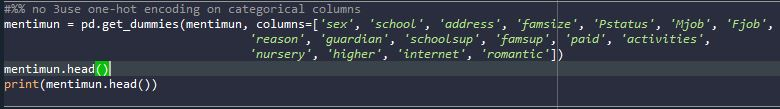
\includegraphics[scale=0.4]{figures/Chap3-1.JPG}
	\caption{Source Code Task 3}
    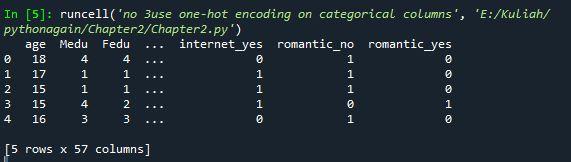
\includegraphics[scale=0.5]{figures/Chap3-1.1.JPG}
	\caption{Hasil Task 3}
\end{figure}

\item shuffle rows
\begin{figure}[!htbp]
    \centering
    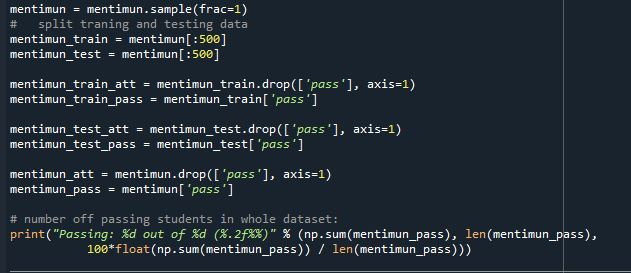
\includegraphics[scale=0.4]{figures/Chap4-1.JPG}
	\caption{Source Code Task 4}
	\newpage
    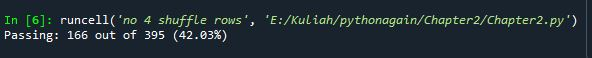
\includegraphics[scale=0.5]{figures/Chap4-1.1.JPG}
	\caption{Hasil Task 4}
\end{figure}

\newpage
\item fit a decision tree
\begin{figure}[!htbp]
    \centering
    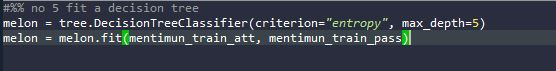
\includegraphics[scale=0.5]{figures/Chap5-1.JPG}
	\caption{Source Code Task 5}
	
    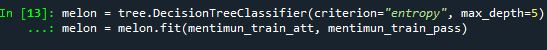
\includegraphics[scale=0.5]{figures/Chap5-1.1.JPG}
	\caption{Hasil Task 5}
\end{figure}


\item visualize tree
\begin{figure}[!htbp]
    \centering
    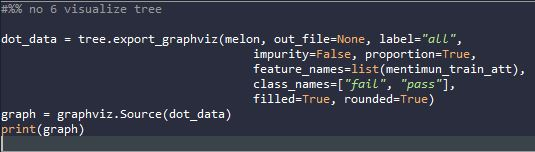
\includegraphics[scale=0.5]{figures/Chap6-1.JPG}
	\caption{Source Code Task 6}
    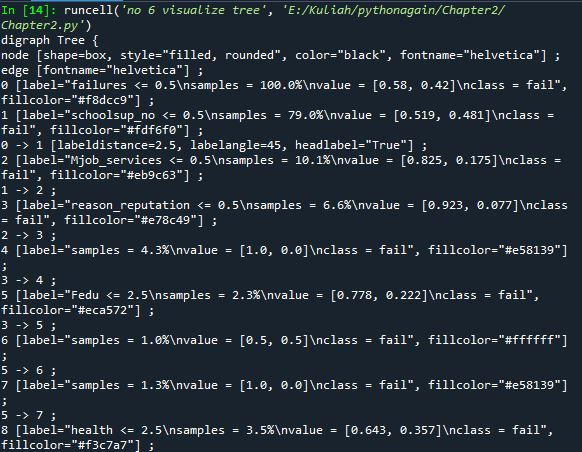
\includegraphics[scale=0.5]{figures/Chap6-1.1.JPG}
	\caption{Hasil Task 6}
\end{figure}

\newpage
\item save tree
\begin{figure}[!htbp]
    \centering
    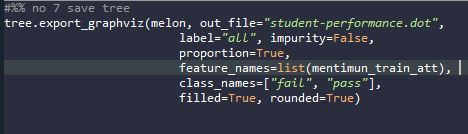
\includegraphics[scale=0.5]{figures/Chap7-1.JPG}
	\caption{Source Code Task 7}
    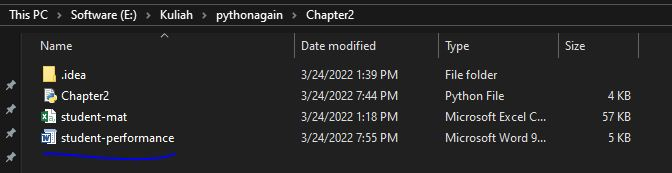
\includegraphics[scale=0.5]{figures/Chap7-1.1.JPG}
	\caption{Hasil Task 7}
    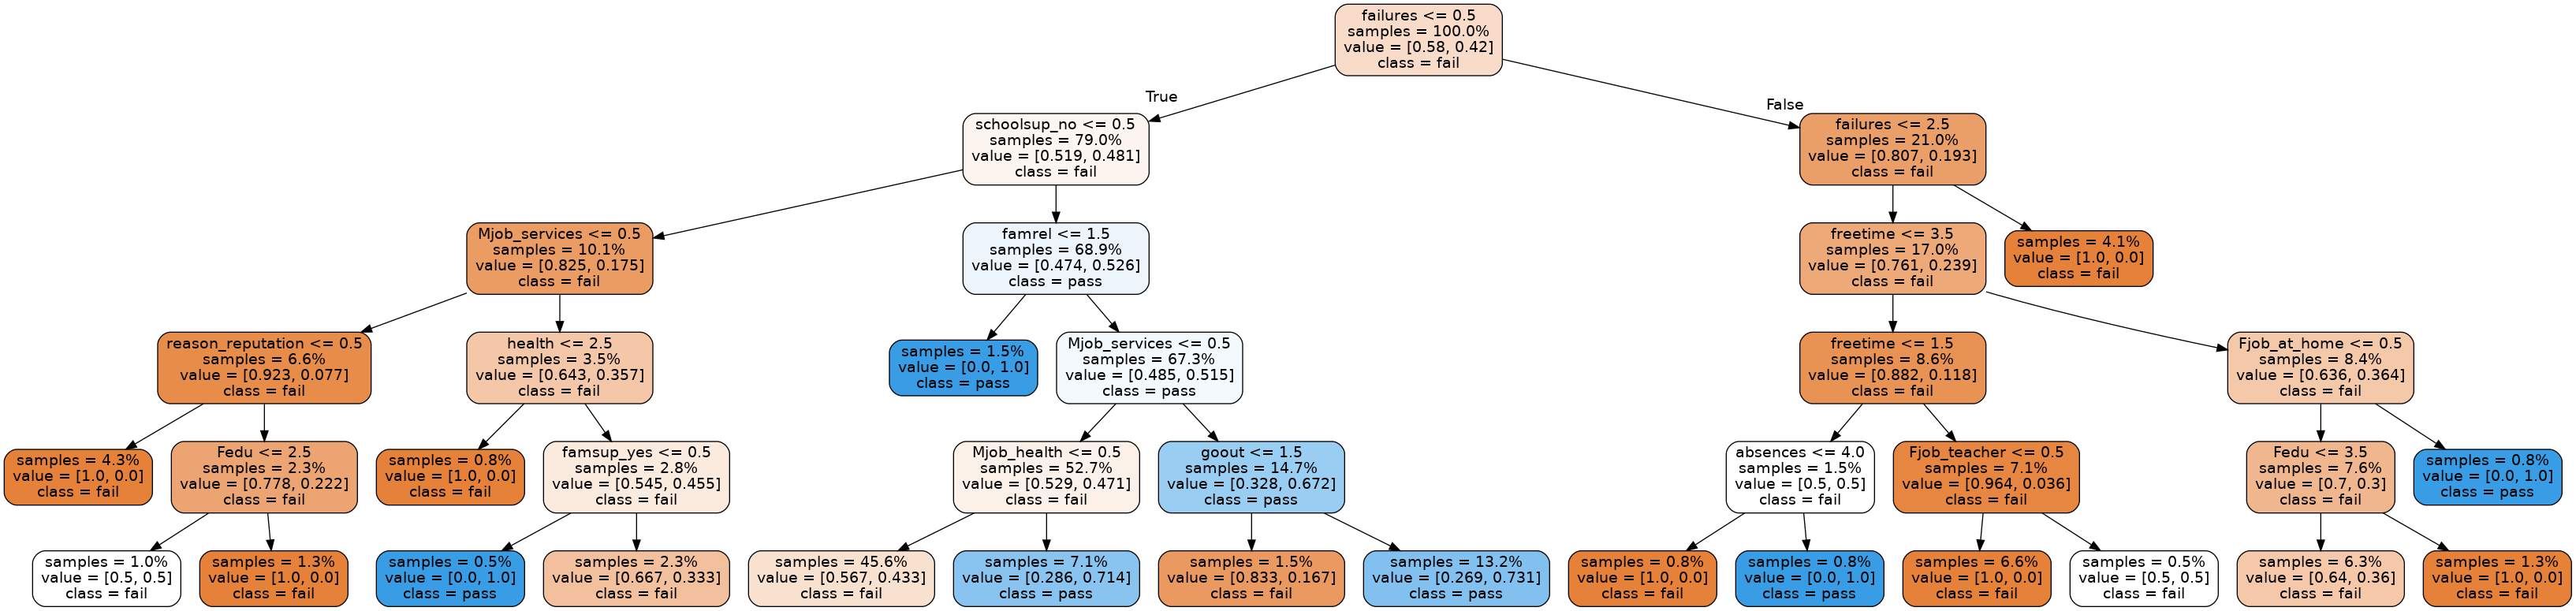
\includegraphics[scale=0.1]{figures/student-performance.png}
	\caption{Hasil Task 7}
\end{figure}

\item task 8
\begin{figure}[!htbp]
    \centering
    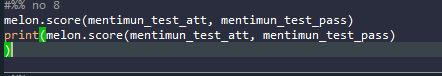
\includegraphics[scale=0.5]{figures/Chap8-1.JPG}
	\caption{Source Code Task 8}
    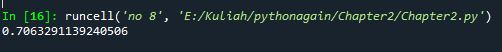
\includegraphics[scale=0.5]{figures/Chap8-1.1.JPG}
	\caption{Hasil Task 8}
\end{figure}


\item task 9
\begin{figure}[!htbp]
    \centering
    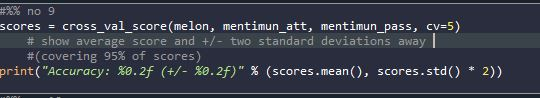
\includegraphics[scale=0.5]{figures/Chap9-1.JPG}
	\caption{Source Code Task 9}
    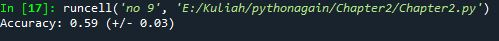
\includegraphics[scale=0.5]{figures/Chap9-1.1.JPG}
	\caption{Hasil Task 9}
\end{figure}

\newpage
\item task 10
\begin{figure}[!htbp]
    \centering
    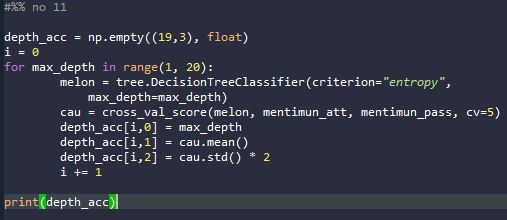
\includegraphics[scale=0.5]{figures/Chap11-1.JPG}
	\caption{Source Code Task 10}
    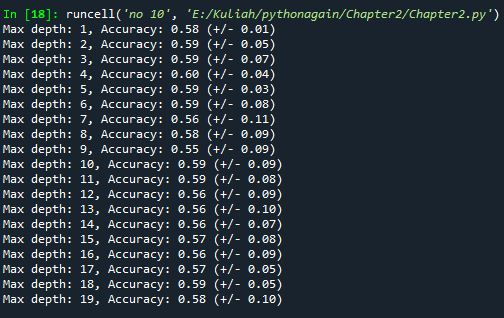
\includegraphics[scale=0.5]{figures/Chap10-1.1.JPG}
	\caption{Hasil Task 10}
\end{figure}


\item task 11
\begin{figure}[!htbp]
    \centering
    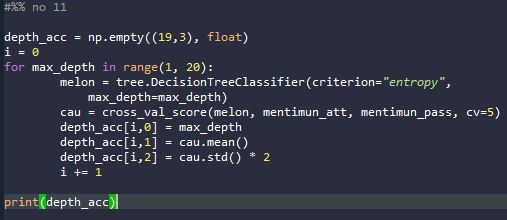
\includegraphics[scale=0.5]{figures/Chap11-1.JPG}
	\caption{Source Code Task 11}
    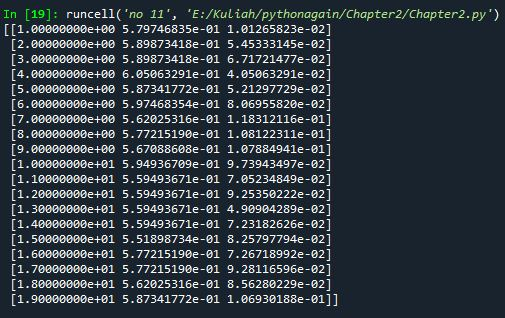
\includegraphics[scale=0.5]{figures/Chap11-1.1.JPG}
	\caption{Hasil Task 11}
\end{figure}

\newpage
\item task 12
\begin{figure}[!htbp]
    \centering
    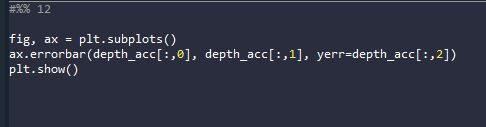
\includegraphics[scale=0.5]{figures/Chap12-1.JPG}
	\caption{Source Code Task 12}
    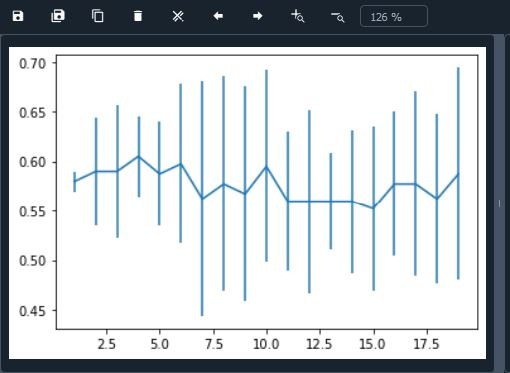
\includegraphics[scale=0.5]{figures/Chap12-1.1.JPG}
	\caption{Hasil Task 12}
\end{figure}

\end{enumerate}


\section{Penanganan Error}
Dari percobaan yang dilakukan di atas, error yang kita dapatkan di dokumentasikan dan di selesaikan(nilai 5 hari kedua):

\begin{enumerate}
	\item
skrinsut error
	\item
Tuliskan kode eror dan jenis errornya
	\item
Solusi pemecahan masalah error tersebut

\end{enumerate}

